\documentclass[10pt,a4paper]{article}
\usepackage[margin=21mm,headheight=15pt]{geometry}
\usepackage[T1]{fontenc}
\usepackage{lmodern,amsmath,amssymb,tikz,graphicx,hyperref,fancyhdr,enumitem}
\usetikzlibrary{arrows.meta,positioning,calc,decorations.pathmorphing}
\definecolor{ink}{RGB}{20,53,78}
\hypersetup{colorlinks=true,urlcolor=ink,linkcolor=ink}
\setlength{\parindent}{0pt}\setlength{\parskip}{5pt}
\emergencystretch=3em
\pagestyle{fancy}\fancyhf{}\fancyfoot[C]{\thepage}
\renewcommand{\headrulewidth}{.3pt}
\newcommand{\task}[2]{\par\medskip{\color{ink}\Large\bfseries #1. #2}\par\smallskip}
\newcommand{\answer}{\par\smallskip\textbf{Worked reasoning.} }
\setlist[enumerate]{label=\textbf{(\alph*)},leftmargin=7mm,itemsep=7pt}
\begin{document}
\fancyhead[L]{\small Control of Dynamical Systems}
\fancyhead[R]{\small Laboratory 10}
{\color{ink}\LARGE\bfseries Laboratory 10}\par
{\large Two thermal zones with one temperature measurement}\par
\textbf{Worked solutions -- five integrated problems}\par
{\small\textbf{Evidence boundary.} Original hypothetical scenarios. Derive, calculate and justify decisions; every numerical record is synthetic. Figures are conceptual and not to scale.}
\smallskip\textbf{Shared nominal data.} Two-zone model: $A=[-0.15,0.05;\,0.05,-0.10]$, $B=[0.1,0]^{\mathsf T}$ and $C=[0,1]$. Feedback pole targets are $-0.20,-0.35$ s$^{-1}$ and observer targets are $-0.8,-1.0$ s$^{-1}$.
\task{1}{Two thermal zones, one heater and one thermometer}
The illustration shows two lumped thermal masses coupled by a conductive bridge. Only zone 1 is heated and only zone 2 is measured.
\begin{center}\resizebox{.80\linewidth}{!}{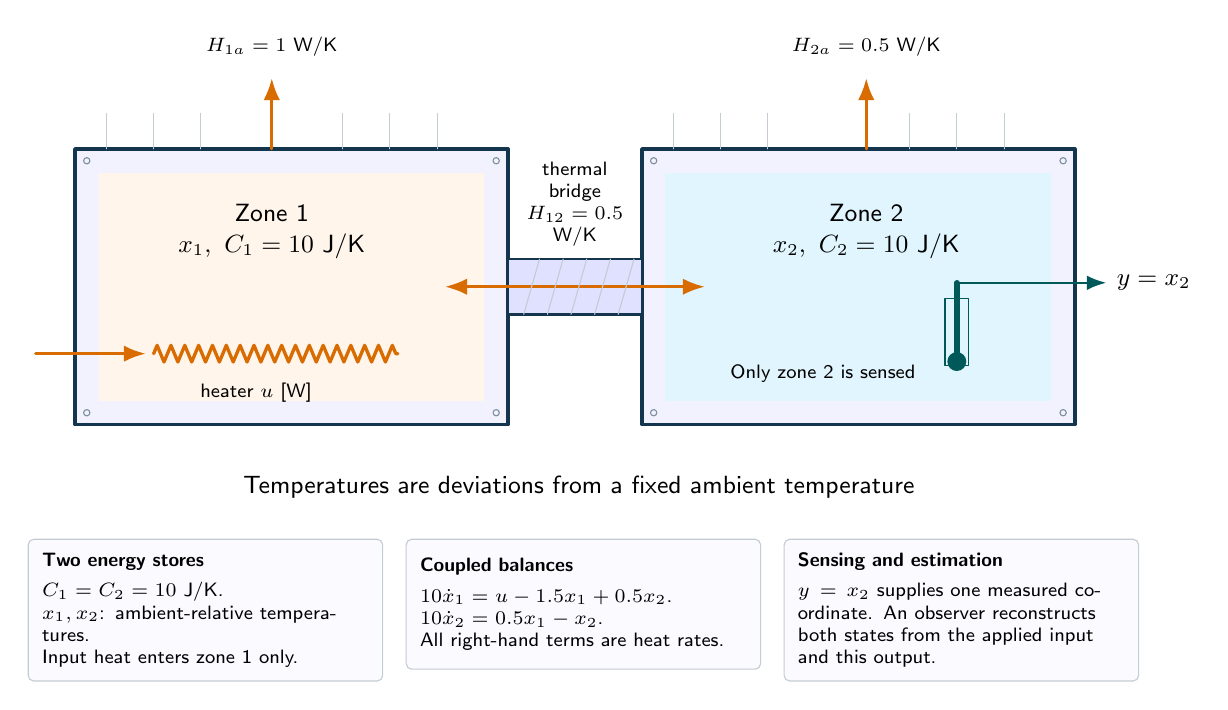
\begin{tikzpicture}[
font=\sffamily\small,>=Latex,line cap=round,line join=round,
wall/.style={draw=ink,line width=1.2pt,fill=blue!5},
water/.style={fill=cyan!25,draw=none},
metal/.style={draw=ink,fill=blue!12,line width=.9pt},
flow/.style={->,draw=blue!65!black,line width=1.2pt},
heat/.style={->,draw=orange!85!black,line width=1.1pt},
measure/.style={->,draw=teal!70!black,line width=.9pt},
dim/.style={<->,draw=ink!65,line width=.6pt},
spring/.style={draw=ink,decorate,decoration={coil,aspect=.5,segment length=4pt,amplitude=3pt}},
wire/.style={draw=ink,line width=1pt},
lab/.style={align=center,font=\sffamily\small},
smalllab/.style={align=center,font=\sffamily\scriptsize}]

\draw[wall](.6,.7)rectangle(6.1,4.2);
\draw[wall](7.8,.7)rectangle(13.3,4.2);
\fill[orange!8](.9,1)rectangle(5.8,3.9);
\fill[cyan!12](8.1,1)rectangle(13,3.9);
\draw[metal](6.1,2.1)rectangle(7.8,2.8);
\draw[heat,<->](5.3,2.45)--(8.6,2.45);
\node[smalllab]at(6.95,3.5){thermal\\bridge\\$H_{12}=0.5$\\W/K};
\draw[orange!85!black,line width=1.2pt,decorate,decoration={zigzag,segment length=5pt,amplitude=3pt}](1.6,1.6)--(4.7,1.6);
\draw[heat](.1,1.6)--(1.5,1.6);
\node[smalllab]at(2.9,1.1){heater $u$ [W]};
\node[lab]at(3.1,3.15){Zone 1\\$x_1,\ C_1=10$ J/K};
\node[lab]at(10.65,3.15){Zone 2\\$x_2,\ C_2=10$ J/K};
\draw[teal!70!black,line width=2pt](11.8,1.5)--(11.8,2.5);
\fill[teal!70!black](11.8,1.5)circle(.12);
\draw[measure](11.8,2.5)--(13.7,2.5)node[right]{$y=x_2$};
\draw[heat](3.1,4.2)--(3.1,5.1);
\draw[heat](10.65,4.2)--(10.65,5.1);
\node[smalllab]at(3.1,5.5){$H_{1a}=1$ W/K};
\node[smalllab]at(10.65,5.5){$H_{2a}=0.5$ W/K};
\node[lab]at(7,-.1){Temperatures are deviations from a fixed ambient temperature};
% REFINED EQUIPMENT DETAILS

% Distinct thermal masses and finite conductive contact.
\foreach \x in {1,1.6,2.2,4,4.6,5.2}{\draw[ink!25](\x,4.2)--(\x,4.65);}
\foreach \x in {8.2,8.8,9.4,11.2,11.8,12.4}{\draw[ink!25](\x,4.2)--(\x,4.65);}
\foreach \x in {6.3,6.6,6.9,7.2,7.5}{\draw[ink!25](\x,2.1)--(\x+.2,2.8);}
\foreach \x/\y in {.75/.85,.75/4.05,5.95/.85,5.95/4.05,7.95/.85,7.95/4.05,13.15/.85,13.15/4.05}{\draw[ink!55](\x,\y)circle(.04);}
\draw[teal!70!black](11.65,1.45)rectangle(11.95,2.3);
\node[smalllab]at(10.1,1.35){Only zone 2 is sensed};

\node[draw=ink!25,fill=blue!2,rounded corners=2pt,anchor=north west,text width=4.15cm,minimum height=1.65cm,inner sep=5pt,align=left,font=\sffamily\scriptsize]at(0.0,-0.75){\textbf{Two energy stores}\\[3pt]$C_1=C_2=10$ J/K.\\$x_1,x_2$: ambient-relative temperatures.\\Input heat enters zone 1 only.};
\node[draw=ink!25,fill=blue!2,rounded corners=2pt,anchor=north west,text width=4.15cm,minimum height=1.65cm,inner sep=5pt,align=left,font=\sffamily\scriptsize]at(4.8,-0.75){\textbf{Coupled balances}\\[3pt]$10\dot x_1=u-1.5x_1+0.5x_2$.\\$10\dot x_2=0.5x_1-x_2$.\\All right-hand terms are heat rates.};
\node[draw=ink!25,fill=blue!2,rounded corners=2pt,anchor=north west,text width=4.15cm,minimum height=1.65cm,inner sep=5pt,align=left,font=\sffamily\scriptsize]at(9.6,-0.75){\textbf{Sensing and estimation}\\[3pt]$y=x_2$ supplies one measured coordinate. An observer reconstructs both states from the applied input and this output.};
\end{tikzpicture}
}\par{\small Two thermal inventories are connected by a conductive bridge. Heating acts in the first zone and sensing in the second. These stated capacities and conductances reproduce the two-state model exactly under the lumped assumptions.}\end{center}
\begin{enumerate}
\item Consider $A=[-0.15,0.05;0.05,-0.10]$, $B=[0.1,0]^T$, $C=[0,1]$. Write both scalar state equations and identify the actuated and measured zones. Find the open-loop poles.
\answer The equations are $\dot x_1=-0.15x_1+0.05x_2+0.1u$ and $\dot x_2=0.05x_1-0.10x_2$, with $y=x_2$. Heating acts in zone 1, while only zone 2 is measured. The characteristic polynomial is $s^2+0.25s+0.0125$, giving roots $(-0.25\pm\sqrt{0.0125})/2$, approximately $-0.18090$ and $-0.06910$. The open-loop model is stable but the slow mode governs long transients.
\item Construct the controllability and observability matrices and evaluate their determinants. Explain the role of inter-zone coupling.
\answer Since $AB=[-0.015,0.005]^T$, controllability is $\mathcal C=\begin{bmatrix}0.1&-0.015\\0&0.005\end{bmatrix}$ with determinant 0.0005. Observability is $\mathcal O=\begin{bmatrix}0&1\\0.05&-0.10\end{bmatrix}$ with determinant $-0.05$. Both ranks are two. The coupling permits the input in zone 1 to affect zone 2 and allows its measurement to carry information about zone 1. Zero coupling would destroy both properties for this input/output placement.
\item Realize the stated matrix using $C_1=C_2=10$ J/K, coupling conductance $H_{12}=0.5$ W/K and ambient conductances $H_{1a}=1$, $H_{2a}=0.5$ W/K. Derive the balances and explain what happens to controllability and observability when coupling is removed.
\answer The balances are $10\dot x_1=u-1x_1-0.5(x_1-x_2)$ and $10\dot x_2=0.5(x_1-x_2)-0.5x_2$. Division by 10 recovers the stated A and B. Removing $H_{12}$ isolates the measured zone from the heater: the actuator cannot influence zone 2 and the sensor cannot reveal zone 1. Each two-state rank test then has rank one. This physical explanation identifies why a nonzero coupling term matters.
\end{enumerate}

\newpage
\task{2}{Pole placement and the distinction between transient and steady feasibility}
First design ideal full-state feedback and its reference prefilter. Then check whether the resulting input request can be delivered by a constrained heater.
\begin{enumerate}
\item Choose $u=-Kx+Nr$ so $A-BK$ has poles $-0.2$ and $-0.35$. Derive K by matching trace and determinant, without a pole-placement library.
\answer Write $K=[k_1,k_2]$. The characteristic polynomial of $A-BK$ is $s^2+(0.25+0.1k_1)s+(0.0125+0.01k_1+0.005k_2)$. The target is $(s+0.2)(s+0.35)=s^2+0.55s+0.07$. Therefore $k_1=3$ and $0.0125+0.03+0.005k_2=0.07$, giving $k_2=5.5$. This explicit matching also checks the sign convention in $u=-Kx+Nr$.
\item With $K=[3,5.5]$, find N for unit DC reference tracking at $y=x_2$. Determine both equilibrium states and input for a unit reference.
\answer At equilibrium the second state equation gives $x_1=2x_2$. Requiring $x_2=r=1$ gives $x=[2,1]^T$. The first physical balance then yields $0=-0.3+0.05+0.1u$, so $u=2.5$. Feedback gives $u=-3(2)-5.5(1)+N$, hence $N=14$. Equivalently $N=-1/[C(A-BK)^{-1}B]$. Nominal reference gain is corrected without adding an integrator.
\item Use $r=0.5$, zero initial states and heater limits $0\le u\le2$ W. Compare the immediate ideal control request with the equilibrium request. Does a feasible equilibrium imply an entirely unsaturated transient?
\answer At $t=0$, $u=Nr-Kx=14(0.5)=7$ W, above the limit. At the nominal equilibrium, $x=[2r,r]^T=[1,0.5]^T$ and $u=2.5r=1.25$ W, within limits. Therefore steady feasibility does not imply transient feasibility. The linear pole-placement prediction assumes unrestricted actuation; the constrained transient must be simulated or designed explicitly.
\end{enumerate}

\newpage
\task{3}{An observer must receive the input actually applied}
Construct the observer and analyze estimated-state feedback. Distinguish the linear separation argument from an implementation with actuator clipping.
\begin{center}\resizebox{\ifdim\width>.98\linewidth.98\linewidth\else\width\fi}{!}{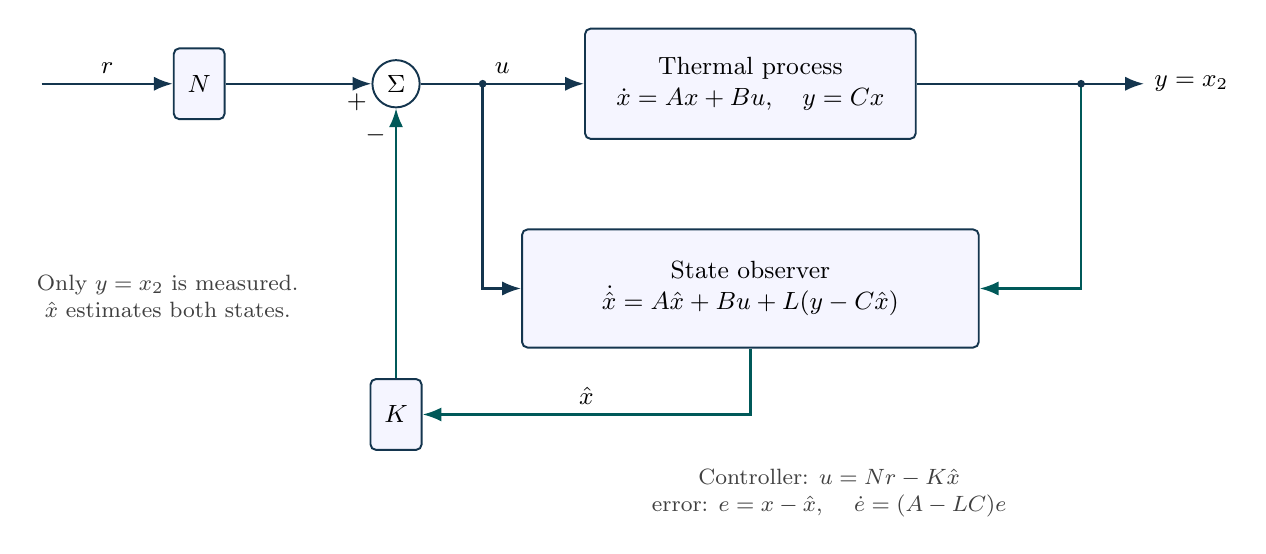
\begin{tikzpicture}[x=1cm,y=1cm,>=Latex,font=\small,
block/.style={draw=ink,fill=blue!4,rounded corners=2pt,minimum height=9mm,align=center,line width=.7pt,inner sep=5pt},
sum/.style={circle,draw=ink,fill=white,minimum size=6mm,inner sep=0pt,line width=.7pt},
sig/.style={->,draw=ink,line width=.85pt},
fb/.style={->,draw=teal!70!black,line width=.85pt},
dist/.style={->,draw=orange!75!black,line width=.85pt},
tap/.style={circle,fill=ink,inner sep=1.4pt},
note/.style={font=\footnotesize,align=center,text=black!75}]

\node[block](n)at(2,1.1){$N$};
\node[sum](u)at(4.5,1.1){$\Sigma$};
\node[block,minimum width=42mm,minimum height=14mm](p)at(9,1.1){Thermal process\\$\dot x=Ax+Bu,\quad y=Cx$};
\draw[sig](0,1.1)--node[above]{$r$}(n);
\draw[sig](n)--node[pos=.9,below]{$+$}(u);
\draw[sig](u)--node[above]{$u$}(p);
\draw[sig](p)--(14,1.1)node[right]{$y=x_2$};
\node[block,minimum width=58mm,minimum height=15mm](o)at(9,-1.5){State observer\\$\dot{\hat x}=A\hat x+Bu+L(y-C\hat x)$};
\draw[sig](5.6,1.1)--(5.6,-1.5)--(o.west);
\fill[ink](5.6,1.1)circle(1.4pt);
\draw[fb](13.2,1.1)--(13.2,-1.5)--(o.east);
\fill[ink](13.2,1.1)circle(1.4pt);
\node[block](k)at(4.5,-3.1){$K$};
\draw[fb](o.south)--(9,-3.1)--node[above]{$\hat x$}(k);
\draw[fb](k.north)--node[pos=.9,left]{$-$}(u.south);
\node[note]at(1.6,-1.6){Only $y=x_2$ is measured.\\$\hat x$ estimates both states.};
\node[note]at(10,-4.1){Controller: $u=Nr-K\hat x$\\error: $e=x-\hat x$, $\quad\dot e=(A-LC)e$};

\end{tikzpicture}
}\par{\small The observer receives both the applied control and measured output. Its estimated vector supplies state feedback; the prefilter sets nominal reference gain.}\end{center}
\begin{enumerate}
\item Use $\dot{\hat x}=A\hat x+Bu+L(y-C\hat x)$ and place observer error poles at $-0.8$ and $-1$. Derive both entries of L.
\answer Let $L=[l_1,l_2]^T$. Then $A-LC=\begin{bmatrix}-0.15&0.05-l_1\\0.05&-0.10-l_2\end{bmatrix}$. Its polynomial is $s^2+(0.25+l_2)s+(0.0125+0.15l_2+0.05l_1)$. Matching $(s+0.8)(s+1)=s^2+1.8s+0.8$ gives $l_2=1.55$ and $l_1=11.1$. The error convention $e=x-\hat x$ yields $\dot e=(A-LC)e$ for the exact model without noise.
\item With estimated-state control $u=-K\hat x+Nr$, derive the augmented dynamics in coordinates $[x,e]$ where $e=x-\hat x$. List all four eigenvalues and state the assumptions.
\answer Since $\hat x=x-e$, the plant evolves as $\dot x=(A-BK)x+BK e+BNr$. The noise-free error obeys $\dot e=(A-LC)e$. Thus the augmented matrix is $\begin{bmatrix}A-BK&BK\\0&A-LC\end{bmatrix}$, whose triangular block structure gives eigenvalues $-0.2,-0.35,-0.8,-1$. The conclusion assumes a matching linear model and the implemented control input available to the observer. Saturation, unknown disturbances or model errors require additional analysis.
\item If the heater saturates, derive the estimation-error dynamics when the observer receives actual applied $u$. Contrast this with feeding it the unlimited request $u_*$. State which linear conclusion no longer follows automatically.
\answer When plant and observer use the same applied $u$, subtraction still gives $\dot e=(A-LC)e$ for the exact noiseless plant, even if the input was produced by saturation. If the observer instead uses $u_*$, then $\dot e=(A-LC)e+B(u-u_*)$, so saturation drives estimation error. The full controlled plant is nonlinear under clipping; the linear block-triangular separation proof no longer establishes its global tracking or stability behavior.
\end{enumerate}

\newpage
\task{4}{Unknown heat leakage, actuator capacity and integral augmentation}
A constant unmodeled heat input enters zone 2. The nominal reference prefilter cannot cancel an unknown disturbance, and additional control action still faces a finite heater limit.
\begin{enumerate}
\item For full-state feedback with the nominal prefilter, add disturbance $d$ to $\dot x_2$. Derive the final output error for a constant d and evaluate it at $d=0.01$.
\answer The perturbed equilibrium is $x=-(A-BK)^{-1}(BNr+Ed)$ with $E=[0,1]^T$. Thus $y=r-C(A-BK)^{-1}Ed$. Here $A-BK=[-0.45,-0.5;0.05,-0.1]$, determinant 0.07, and $C(A-BK)^{-1}E=-0.45/0.07=-45/7$. Therefore $y-r=(45/7)d$. At 0.01, the offset is $9/140\approx0.064286$. A nominal static prefilter does not reject an unknown constant disturbance.
\item Assume heater command must stay in $[0,2]$. Under the nominal model, determine the largest positive constant zone-2 reference that full-state control can maintain at equilibrium. Explain the implication for a requested reference of one.
\answer From the physical balances at a reference r, $x_2=r$, $x_1=2r$ and $u=2.5r$. Therefore $r\le2/2.5=0.8$. A unit reference requires 2.5 and is infeasible. Nominal pole placement and prefilter calculations do not enforce actuator constraints. A controller can be mathematically stable in its unlimited model while failing to attain a constrained operating point.
\item Propose an integral state for rejecting an unknown constant output error and write the augmented plant matrices before gain design. Check whether the nominal augmented model is controllable, and explain what augmentation cannot fix.
\answer Set $\dot z=r-Cx$ and use augmented state $[x^T,z]^T$. For gain design, $A_a=\begin{bmatrix}A&0\\-C&0\end{bmatrix}$ and $B_a=\begin{bmatrix}B\\0\end{bmatrix}$. The controllability determinant is $-2.5\times10^{-6}$ for the stated ordering, hence the nominal three-state model is controllable. Integral feedback can reject feasible constant disturbances when the resulting loop is stable. It cannot make the nominal 1 K target feasible with only 2 W; that equilibrium needs 2.5 W.
\end{enumerate}

\newpage
\task{5}{Fast estimation, biased sensors and the limits of a noise-path calculation}
Observer poles are chosen faster than controller poles. Examine both modal time scales and the effect of measurement noise without claiming that faster poles improve every error norm.
\begin{enumerate}
\item Let measured output be $y_m=Cx+n$. Derive the estimation-error dynamics with noise. Then, with true state and input held at zero, derive the transfer from n to the estimate of zone 2 for the selected observer.
\answer Subtracting observer from plant gives $\dot e=(A-LC)e-Ln$. With true state and input held at zero, $\dot{\hat x}=(A-LC)\hat x+Ln$. The second row of $(sI-A+LC)^{-1}L$ gives $\hat X_2/N=[0.05(11.1)+(s+0.15)1.55]/[(s+0.8)(s+1)]$, or $(1.55s+0.7875)/(s^2+1.8s+0.8)$. Its DC gain is 0.984375. This isolated observer transfer is distinct from the full closed-loop noise-to-output transfer.
\item Compare the slowest controller and observer modal time constants. Explain why a faster observer pole does not by itself guarantee the same proportional decrease in every estimation-error norm at every time.
\answer The slowest feedback pole is $-0.2$, with time constant 5 s. The slowest observer pole is $-0.8$, with time constant 1.25 s, a factor of four faster by this modal measure. Individual modes decay exponentially, but total error depends on modal coefficients, initial conditions, eigenvector conditioning and measurement noise. Pole locations alone do not order every finite-time norm. The selected observer also has a second pole at $-1$ and nontrivial coupling between states.
\item Hold the true state and input at zero and add constant sensor bias $n=0.1$ K. Find both steady state estimates for the chosen observer. Explain why this open estimator test does not directly give the final output of the fully closed loop.
\answer The steady estimate is $-(A-LC)^{-1}Ln$. The two DC gains are $1.1875/0.8=1.484375$ and $0.7875/0.8=0.984375$, giving $\hat x=[0.1484375,0.0984375]^T$ K. In this test the true input is held at zero. Once estimated-state feedback is closed, the estimate alters the actuator input and the true temperatures; the joint closed-loop noise transfer must then be analyzed. The isolated observer transfer is not that joint transfer.
\end{enumerate}

\end{document}
